
\documentclass{eecslides}

% \usecolortheme{RimouskiDark}

\usepackage[english]{babel}
\usepackage{lipsum}
\usepackage{graphicx}
\usepackage{caption}
\usepackage{hyperref}
\usepackage{xcolor}
\usepackage[round,authoryear]{natbib}
\usepackage[protrusion=true,expansion=true]{microtype}

\title[Data Storage]{Data conservation - Perspectives, issues and solutions.}
\author[M. B. \& S. V.]{\color{white}  Miranda Bryant and Steve Vissault}
\website{\color{white} s.vissault@yahoo.fr}
\institute[\color{white} UQAR]{\color{white} \textbf{Les midis numériques}}
\date{ \color{white} \today}

\setbeamersize{text margin left=1cm} 
\setbeamersize{text margin right=1cm} 
\setbeamersize{text margin top=0.1cm} 

\begin{document}

\begin{frame}[plain]
\titlepage
\end{frame}


%%%%%%%%%%%%%%%%
\section{Introduction}
%%%%%%%%%%%%%%%%

\begin{frame}{Introduction}{Context}

All biologists collect data during their career but most of them are using \alert{inapropriate files} to long term storage:

\begin{itemize}
	\item  Open Office or Microsoft spreadsheet
	\item  text and CSV files
\end{itemize}

\textbf{Some risks attributes at those practices:} Overwriting file, lost the full dataset or some records.

\end{frame}

%%%%%%%%%%%%%%%%%%%%%%%%%%%%%%%%%%%%%%%%%%%%%%%%%%%%%%%%

\begin{frame}{Introduction}{Context}

\textbf{\alert{Disadvantage of classic storage file (ex. Excel)}}

\begin{enumerate}
	\item Flat file
	\item No dynamic query, only filters
	\item Large dataset could be messy
	\item Exportability %Files corrupted, plateform could be different between users
	\item Absence of fonctionnality on manage multiple users
	\item Missing options to create metadata
\end{enumerate}

%% Basic question for the public: How many people generate a dynamic cross table on Excel and got twice the same word because the first one start by a capital letter and the second doesn't start by a capital letter ?

%% Define briefly what's a medata file ?

\end{frame}


%%%%%%%%%%%%%%%%
\section{Why do something different ?}
%%%%%%%%%%%%%%%%


\begin{frame}{Why do something different ?}{Data lost}


\begin{columns}[c]
	\begin{column}{.50\paperwidth}
		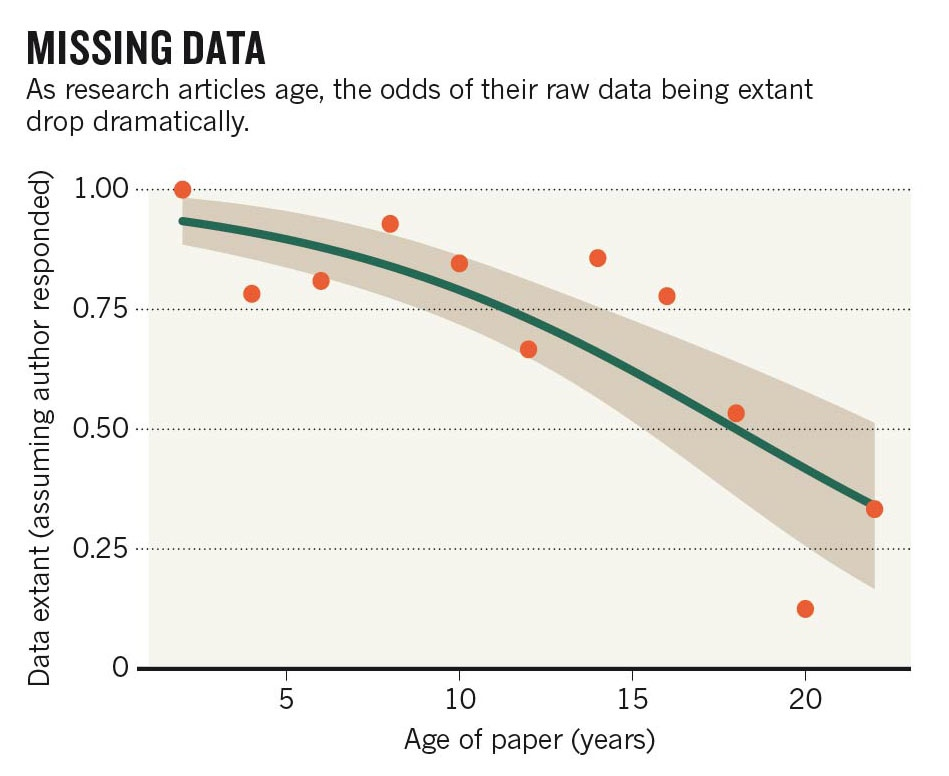
\includegraphics[width=.50\paperwidth]{Nature_fig.jpg}
	\end{column}
	\begin{column}{.4\paperwidth}
		 Data for almost all studies published just two years ago were still accessible, the chance of them being so \alert{fell by 17\% per year} \citep{Vines2013}
	\end{column}
\end{columns}


\end{frame}

%%%%%%%%%%%%%%%%%%%%%%%%%%%%%%%%%%%%%%%%%%%%%%%%%%%%%%%%

\begin{frame}{Why do something different ?}

\textbf{We need to keep focus on those points as a part of our biologist culture:}
	
	\begin{itemize}
		\item \alert{All datasets} containing specific information given a time and a location \alert{are usefull}.
		\item 80\% of datasets are built on \alert{public funding} \citep{Graham2013} and should be accessible publicly
		\item All datasets could be re-used, recycle or valorize (as the 3-R in waste management: Reduce, Reuse, Recycle) 
	\end{itemize}


\end{frame}

%%%%%%%%%%%%%%%%
%% References
%%%%%%%%%%%%%%%%

\nocite{Poisot2013a}

\begin{frame}[allowsframebreaks]{Reference}
	\bibliographystyle{abbrvnat}
	\bibliography{/home/steve/Dropbox/Bibtex/OpenAccess}	
\end{frame}

\end{document}